%%%%%%%%%%%%%%%%%%%%%%%%%%%%%%%%%%%%%%%%%%%%%%%%%%%%%%%%%%%%%%%%%%%%%%%%
% Escuela Politécnica Superior de la Universidad de Alicante
% Realizado por: Jose Manuel Requena Plens
% Contacto: info@jmrplens.com / Telegram:@jmrplens
%%%%%%%%%%%%%%%%%%%%%%%%%%%%%%%%%%%%%%%%%%%%%%%%%%%%%%%%%%%%%%%%%%%%%%%%

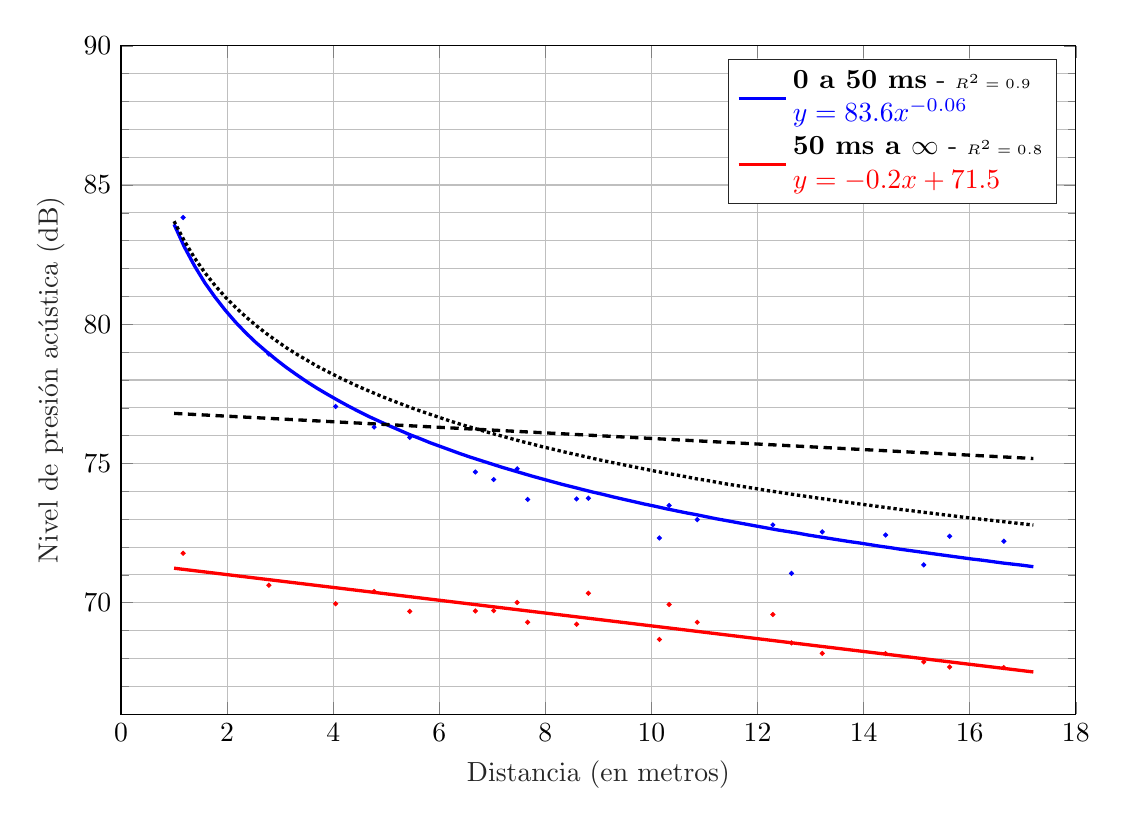
\begin{tikzpicture}

\begin{axis}[%
width=\textwidth,
height=0.7\textwidth,
at={(0\textwidth,0\textwidth)},
scale only axis,
xmin=0,
xmax=18,
xlabel style={font=\color{white!15!black}},
xlabel={Distancia (en metros)},
ymin=66,
ymax=90,
ylabel style={font=\color{white!15!black}},
ylabel={Nivel de presión acústica (dB)},
axis background/.style={fill=white},
xmajorgrids,
xminorgrids,
ymajorgrids,
yminorgrids,
minor y tick num= 4,
legend style={legend cell align=left, align=left, draw=white!15!black}
]
% Curvas CATT
\addplot[color=blue,domain=1:17.2, samples=85,line width=1.2]{83.59*x^(-0.056)};
\addlegendentry{\textbf{0 a 50 ms} - \tiny{$R^2 = 0.9$}\\$\color{blue}y = 83.6·x^{-0.06}$}

\addplot[color=red,domain=1:17.2, samples=85,line width=1.2]{-0.23*x+71.47};
\addlegendentry{\textbf{50 ms a $\infty$} - \tiny{$R^2 = 0.8$}\\$\color{red}y = -0.2·x+71.5$}

% Curvas insitu
\addplot[color=black,densely dotted,line width=1.2pt,domain=1:17.2, samples=85]{82.4*x^(-0.05)+1.3};
\addplot[color=black,densely dashed,line width=1.2pt,domain=1:17.2, samples=85]{-0.1*x+75.6+1.3};

% Puntos
\addplot [color=blue, only marks,mark size=0.7pt]
  table[row sep=crcr]{%
1.17046999107196	83.8329777120332\\
2.78747197295327	78.9306384962613\\
4.04598566482878	77.0498042019777\\
4.77179211617606	76.3062472099297\\
5.44357419348722	75.9377982206261\\
6.68075594525051	74.6944529453703\\
7.02637886823647	74.4249636604886\\
7.46793144049944	74.8080290478306\\
7.66615940350838	73.7111005477617\\
8.58894638474359	73.7286958740670\\
8.81093071133805	73.7544124640849\\
10.1498768465435	72.3277287217195\\
10.3329569823938	73.4949762336248\\
10.8637010268140	72.9838872461474\\
12.2890194889584	72.7960325948105\\
12.6400158227749	71.0558026132494\\
13.2200605142337	72.5464433961370\\
14.4142290810157	72.4316131041346\\
15.1334067545943	71.3605121070253\\
15.6211395230950	72.3863346098596\\
16.6439178080162	72.2106523500810\\
18.4775539506722	72.3500886557943\\
};

\addplot [color=red, only marks,mark size=0.7pt]
  table[row sep=crcr]{%
  1.17046999107196	71.7775654046139\\
2.78747197295327	70.6303063464095\\
4.04598566482878	69.9635797822371\\
4.77179211617606	70.4020975986096\\
5.44357419348722	69.6894116908404\\
6.68075594525051	69.7053811912342\\
7.02637886823647	69.7137208542767\\
7.46793144049944	70.0108618230364\\
7.66615940350838	69.3018030921320\\
8.58894638474359	69.2302641444601\\
8.81093071133805	70.3403117898067\\
10.1498768465435	68.6839446505491\\
10.3329569823938	69.9369892497103\\
10.8637010268140	69.2995548128369\\
12.2890194889584	69.5772033188763\\
12.6400158227749	68.5595087780777\\
13.2200605142337	68.1835354842376\\
14.4142290810157	68.1753790141965\\
15.1334067545943	67.8793448780429\\
15.6211395230950	67.6907594619848\\
16.6439178080162	67.6707394060713\\
18.4775539506722	66.8649481024522\\
  };
\end{axis}
\end{tikzpicture}%